\begin{figure}[t]
    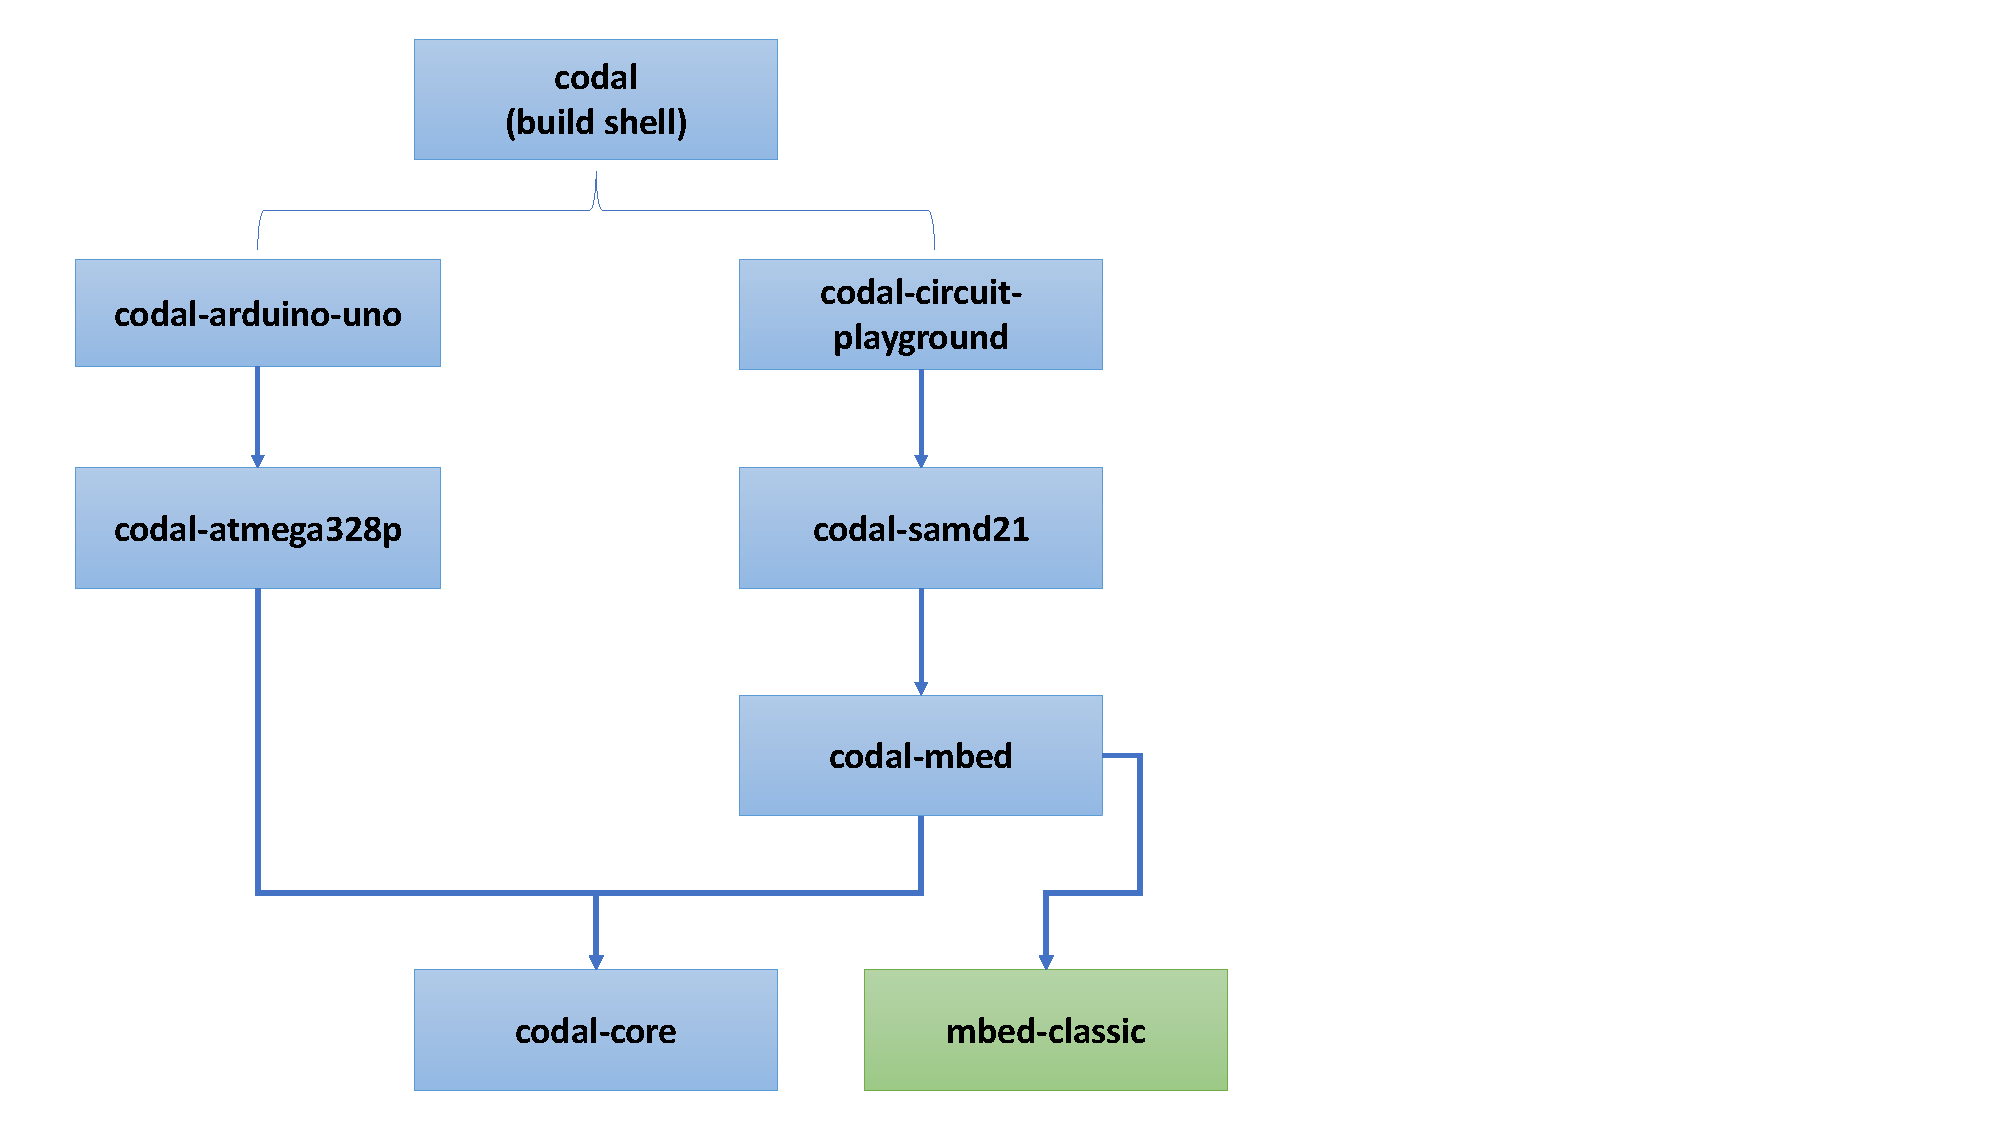
\includegraphics[width=4.5in]{codalFig.pdf}
    \caption{\label{fig:codal}Detailed relationships between \CO repos.}
\end{figure}

\section{The \CO Runtime}
\label{sec:codal}

\CO is a component-oriented device runtime designed to make efficient use of memory and energy, provide both synchronous and asynchronous API variants, and be a reasonable target for higher level languages such as JavaScript.  It is the preferred runtime
for \MC and, as such, is supported by an annotated C++ library (\emph{\MCN-common-packages}) defining and abstracting
the mapping from \CO to TypeScript. The use of \MCN-common-packages ensures that different \MC targets that 
use \CO share a common Typescript and block API vocabulary.

\CO provides a set of components that abstract away microcontroller specifics, a non-preemptive scheduler that minimizes the need for resource locking primitives whilst allowing asynchronous operation, and an eventing subsystem (common to all components) that enables the decoupling of system and user code.

\CO components represent software or hardware drivers (e.g., an I2C device, a GPIO pin, a Message Bus, a Bluetooth device); any component can generate or consume events. \CO supports both polling and asynchronous (event-driven) programming models, which enables higher level languages to map straight onto native C/C++ APIs. Section~\ref{sec:related} compares \CO to other runtimes and operating systems for microcontrollers.

% more required here, needs to be reflowed...

\subsection{Structural Overview}

\begin{figure}
% TODO: shrink width
\begin{lstlisting}
class ArduinoUno : public RTDevice
{
    ...
    public:
        ATMegaTime       timer;
        ATMegaSerial     serial;
        ATMegaI2C        i2c;
        MessageBus       messageBus;

        ArduinoUno();
};
\end{lstlisting}
\caption{\label{fig:codalSingleton}Singleton for Arduino Uno}
\end{figure}

Figure~\ref{fig:codal} shows the repository architecture for two \CO devices, the Adafruit CircuitPlayground, built on top of ARM's Mbed, and the Arduino Uno, built without any supporting libraries. The \COLN-core repo sits at the base of both device trees and provides the high level driver models which are implemented in the layer above. Each target library (\COLN-arduino-uno, \COLN-circuit-playground) builds on top of a processor library containing processor specific files, and the target library at the top of the tree contains files specific to a device --- commonly the linker script and the model for a device. A model is a C++ class that brings together components defined further down the tree as a single software representation of the device,
as shown in Figure~\ref{fig:codalSingleton}.
This architecture enables platform independent code to run across multiple processors and devices, while allow for extensibility and specialization.

\subsection{Message Bus and Events}

Message passing via events is a common technique and is the foundation of many operating systems --- yet in most systems events are static, used only to notify users of key events within the system (e.g. SIGKILL on UNIX).

\CO offers extensible events where the data contained in an event can be arbitrary, and application specific. Application developers can then ``listen'' to events, specifying an id (namespace), a value (unique within a namespace), and a function to be invoked when an event is raised. All events pass through the message bus: if a corresponding listener is in place, the function indicated by the listener is invoked. The eventing model aligns well to JavaScript and languages with event-based programming models.

Not only do events enable easy modularization of code, but they also safeguard the application programmer from situations where incorrect code could cause unexpected behavior. Take for example an application to detect a button press, there are usually two solutions: (1) poll the state of a pin; or (2) configure an interrupt to fire when the state of a pin changes.

\begin{figure}
\begin{lstlisting}
int state = 0;

void buttonClicked() {
    int gpioState = PIN0;
    // button released, blink LED!
    if(state == 1 && gpioState == 0) {
        set_state(LED, 1);
        wait_ms(1000);
        set_state(LED, 0);
    }
    state = gpioState;
}

int main() {
    configure_interrupt(PIN0, buttonClicked);
    while(1);
}
\end{lstlisting}
\caption{\label{fig:pollPin}Pseudocode for detecting a pin transition using interrupts.}
\end{figure}

Figure~\ref{fig:pollPin} shows an example of polling.
This code is considered bad practice as it prevents other interrupts (like Timers) from firing for at least a second when a button is released, however, this is often the first application that a user will create. Such frameworks advise users to avoid blocking functions and waiting in interrupt context, thus sidestepping the problem by punting responsibility to the user --- \CO uses the message bus abstraction to shield users from such scenarios, as shown in Figure~\ref{fig:messageBus}. Note that the user doesn't have to configure any interrupts, as they are handled by pre-existing drivers.

\begin{figure}
\begin{lstlisting}
#include "CircuitPlayground.h"
CircuitPlayground cplay;

void buttonClicked() {
    cplay.io.led.setDigitalValue(1);
    cplay.sleep(1000);
    cplay.io.led.setDigitalValue(0);
}

int main() {
    cplay.messageBus.listen(ID_BUTTON_A,DEVICE_BUTTON_EVT_CLICK,buttonClicked);

    while(1) cplay.sleep(100);
}
\end{lstlisting}
\caption{\label{fig:messageBus}Using the message bus.}
\end{figure}

% Stuff to add (it's already quite long):
% * Provides a similar mechanism seen in higher level languages
% * Timer and queues?
% * message passing microkernel

\subsection{Fiber Scheduler}
% TODO: add Fork on block
Novice users often want to perform multiple operations concurrently, generally requiring threads. \flameon{TBALL: I don't think that it's that they `want` to do it - it's more that the event-based paradigm leads naturally to concurrency, especially in a reactive setting, like that of the microcontroller.}
Threading is a confusing concept: users must learn about locks, semaphores, and preemption, to prevent race conditions. Threads can also consume many resources, depending on the model that is adopted by the runtime environment.

\CO takes a non-preemptive scheduling approach which reduces the need for resource locking primitives. \CO fibers (lightweight threads) are RAM efficient and have a variable stack size. As we adopt a non-preemptive scheduling model, user or driver code must call ``sleep'' to swap context to another fiber, this means that at an invoke of sleep, the stack depth is small. When a fiber is paged out the entire stack is duplicated to the heap. This would normally be ill-advised, but due to a usually small stack size, this is more efficient than approaches where there is a mandated stack size.

Events and the message bus are integral to \CON, even extending to fibers, which can block and wait on events to complete. \flameon{TBALL: this is not much of a sentence - please revise.}

\subsection{Drivers}

Drivers are commonly programmed via low-level interfaces that control external or integrated hardware on a device. For embedded developers, creating and using drivers involves translating datasheets into program code and using such interfaces, which can confuse novice programmers.

\CO drivers abstract away the complexities of the underlying hardware into reusable, extensible, easy-to-use components: for every hardware component there is a software component. \CO has three types of drivers:
\begin{itemize}
    \item[1.] an abstract specification of a driver model common to most devices (e.g. I2C, Serial);
    \item[2.] a driver that relies only on the interfaces specified in a driver model  (e.g. an I2C based driver);
    \item[3.] the concrete implementation of the abstract driver model, which may be platform specific or platform agnostic.
\end{itemize}
Not all devices are the same, and by generalizing the interface, devices can introduce platform specific optimizations and specializations.

Interrupts are integral to drivers: in serial communications it is useful to know when a byte has been sent or received. As illustrated in the button example, performing operations in interrupt context can be detrimental to the device. \CO drivers use events to decouple computational tasks, that may take a variable length of time, from interrupt context.

% * motivation
% * example - I2C, microphone (DMA)
% * one component per piece of hardware or software
% * Provides a common interface
% * uses events to decouple from interrupt context.

\subsection{Memory Management}

Standard libraries in C++ do not offer reentrant versions of memory allocation calls like ``malloc'' and ``new'', forbidding the allocation of memory in interrupt context.

\CO implements its own heap allocator that is designed to safeguard users from the scenario above, introducing reentrant versions of malloc. The heap allocator is flexible and reconfigurable, allowing the specification of multiple heaps across memory and it is optimised for common sizes and repeat allocations.

\CO has a number of managed types that use reference counting to determine when memory should be freed. Internally, managed types use malloc to copy stack allocated data to the heap creating a safer environment for the user --- the reentrant behaviour of malloc and free are key here, as references can be created and destroyed regardless of processor context.
% * provides an interrupt safe environment for memory allocation
% * flexible implementation
%     - multiple heaps
%     - reconfigurable, repurposeable
% * optimisations for common sizes and repeated patterns
% * edu
% * couple of sentences on types
%     - ref counted, malloced types.


